\section{Design Overview}
The design seeks to randomize the mapping from addresses to sets in the cache. We leverage the shorter lifetimes of pages in the cache to give us a periodic change in the hashing scheme used to index into the cache. The design involves using a lookup table, that is indexed using the lower bits of the virtual page number. This gives us the hashing scheme to be used by all addresses that map to that entry. The hash employed is different for different addresses, as the hashing scheme involves using a swizzle of certain bits from the tag. The hash obtained after the application of the hashing scheme to the address is XOR'ed with the original index bits to generate the new cache set index. This ensures a many to many mapping from the set index obtained using original index bits and index generated after the application of the hash. 
\subsection{Hashing scheme (broad ideology)}
\subsection{Hash lifetimes: Variation with entries}
\subsection{Cache Design Used}
The design used here is the recently proposed VC-DSR virtual cache design \cite{}. The primary design philosophy behind this cache is to cache data indexed by an address from a primary or a leading virtual page, where the leading virtual page refers to the page that is cached first, and any synonymous access is remapped to the corresponding address from the leading virtual page.  This design inherently keeps track of the virtual pages currently present in the cache, facilitating the maintenance of hashing schemes while a virtual page is alive in the cache, and their subsequent recycling upon their exit from the cache. Additionally, the use of virtual cache allows us to hide the latency associated with the lookup of the table containing the hashing schemes by overlapping the lookup of the table with the process of generating the effective address. 

\subsection{Issues with Virtually Indexed Physically Tagged Caches}
For a virtually indexed physically tagged cache, application of such a scheme becomes more complicated. This is because synonymous addresses would get hashed differently, because bits in the virtual page number are used to index the table containing the hashing scheme to be used. These bits would be different for synonymous addresses, resulting in them using different hashing schemes. The other option would be to use bits in the physical page number to index the table containing the hashing schemes, however this would defeat the purpose of using a virtually indexed and physically tagged cache, because we would have to wait for the virtual to physical translation to complete, before we could generate the cache set index. If the same hashing scheme was applied to all sets, then the scheme would involve using bits from the physical tag, again involving waiting for the virtual to physical translation to complete. 
\subsection{Issues with Physically Indexed Physically Tagged Caches}
Talk about having to wait address translation to be complete before we can 
proceed to perform the hash table lookup, hence we don't have a way to tolerate the latency
introduced by the table lookup. 
\begin{figure}
  \center{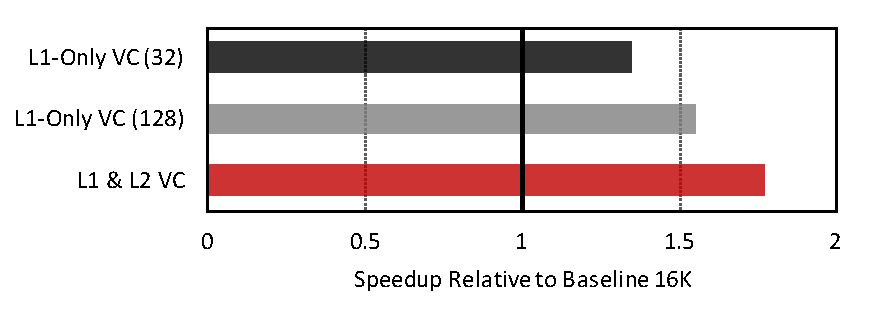
\includegraphics[width=0.95\linewidth]
    {figures/L1VC.pdf}}
  \caption{Proposed GPU virtual cache hierarchy.}
  \label{figure:VCDSR_GPU}
\end{figure}
\subsection{Tolerating introduced latency}
\subsection{Issues with present scheme(not one-to-one and increased tag size)}
Given that the mapping from set number obtained from the set index bits of the original address to the actual set in which the data item is cached is many to many, the original tag bits alone would not suffice to uniquely identify the addresses that get mapped to the particular set. This would entail having to use larger tags in the L1 cache. In effect, because of the many to many mapping from original set number to the mapped set number, our tag size increases to the size of a tag in a fully associative cache. However, the tag comparison is still to be performed only amongst the tags present in the particular set of interest.   <Roughly quote the amount of 

